% \VignetteIndexEntry{The otsad Package: Online Time-Series Anomaly Detectors}
% \VignetteDepends{otsad}
% \VignetteKeywords{otsad}
% \VignetteKeywords{anomaly time serie}
% \VignettePackage{otsad}
%\VignetteCompiler{knitr}
%\VignetteEngine{knitr::knitr}

\documentclass[a4paper]{article}\usepackage[]{graphicx}\usepackage[]{color}
% maxwidth is the original width if it is less than linewidth
% otherwise use linewidth (to make sure the graphics do not exceed the margin)
\makeatletter
\def\maxwidth{ %
  \ifdim\Gin@nat@width>\linewidth
    \linewidth
  \else
    \Gin@nat@width
  \fi
}
\makeatother

\definecolor{fgcolor}{rgb}{0.345, 0.345, 0.345}
\newcommand{\hlnum}[1]{\textcolor[rgb]{0.686,0.059,0.569}{#1}}%
\newcommand{\hlstr}[1]{\textcolor[rgb]{0.192,0.494,0.8}{#1}}%
\newcommand{\hlcom}[1]{\textcolor[rgb]{0.678,0.584,0.686}{\textit{#1}}}%
\newcommand{\hlopt}[1]{\textcolor[rgb]{0,0,0}{#1}}%
\newcommand{\hlstd}[1]{\textcolor[rgb]{0.345,0.345,0.345}{#1}}%
\newcommand{\hlkwa}[1]{\textcolor[rgb]{0.161,0.373,0.58}{\textbf{#1}}}%
\newcommand{\hlkwb}[1]{\textcolor[rgb]{0.69,0.353,0.396}{#1}}%
\newcommand{\hlkwc}[1]{\textcolor[rgb]{0.333,0.667,0.333}{#1}}%
\newcommand{\hlkwd}[1]{\textcolor[rgb]{0.737,0.353,0.396}{\textbf{#1}}}%
\let\hlipl\hlkwb

\usepackage{framed}
\makeatletter
\newenvironment{kframe}{%
 \def\at@end@of@kframe{}%
 \ifinner\ifhmode%
  \def\at@end@of@kframe{\end{minipage}}%
  \begin{minipage}{\columnwidth}%
 \fi\fi%
 \def\FrameCommand##1{\hskip\@totalleftmargin \hskip-\fboxsep
 \colorbox{shadecolor}{##1}\hskip-\fboxsep
     % There is no \\@totalrightmargin, so:
     \hskip-\linewidth \hskip-\@totalleftmargin \hskip\columnwidth}%
 \MakeFramed {\advance\hsize-\width
   \@totalleftmargin\z@ \linewidth\hsize
   \@setminipage}}%
 {\par\unskip\endMakeFramed%
 \at@end@of@kframe}
\makeatother

\definecolor{shadecolor}{rgb}{.97, .97, .97}
\definecolor{messagecolor}{rgb}{0, 0, 0}
\definecolor{warningcolor}{rgb}{1, 0, 1}
\definecolor{errorcolor}{rgb}{1, 0, 0}
\newenvironment{knitrout}{}{} % an empty environment to be redefined in TeX

\usepackage{alltt}
\usepackage[utf8]{inputenc}
\usepackage[T1]{fontenc}
\usepackage{amsmath,amssymb,array}
\usepackage{booktabs}

% Size of the layout
\usepackage[a4paper, total={160mm, 247mm}]{geometry}

%% load any required packages here

\usepackage{color}
\usepackage{stmaryrd}
\usepackage{url}
\usepackage[numbers,sectionbib]{natbib}

\usepackage{authblk}
\usepackage{epstopdf}

\usepackage{booktabs}
\usepackage{multirow}
\IfFileExists{upquote.sty}{\usepackage{upquote}}{}
\begin{document}

\providecommand{\pkg}[1]{\textbf{#1}}
\providecommand{\CRANpkg}[1]{\textbf{#1}}
\providecommand{\code}[1]{\texttt{#1}}
\providecommand{\file}[1]{\texttt{'#1'}}

\title{The \pkg{otsad} Package:\\ Online Time-Series Anomaly Detectors}

%\author{Alaiñe Iturria}

\author[1,2]{Alaiñe Iturria}
\author[2]{Jacinto Carrasco}
\author[2]{Francisco Herrera}
\author[1]{Santi Charramendieta}
\author[1]{Karmele Intxausti}

\affil[1]{IK4-Ikerlan, Big Data Architectures Team, Paseo J.Mª Arizmediarrieta, 2, 20500 Arrasate-Mondragon. Spain}
\affil[2]{Department of Computer Science and Artificial Intelligence, University of Granada, Granada, 18071, Spain}


\date{}

\maketitle

\definecolor{highlight}{rgb}{0,0,0}


\abstract{
Anomaly detection gives valuable information that can be used to solve malfunctions and prevent future problems. Although this field has been widely studied, due to the continuous evolution of technology, new challenges arise that require further improvement and evolution of anomaly detection techniques. In this paper, we present the \pkg{ostad} package that implements six of the most recent detection algorithms capable of dealing with various challenges, such as online and non-stationary univariate time-series anomaly detection.
}

\section{Introduction}

Anomaly detection consists of the identification of patterns in the data that differ from expected behavior and is a relevant task in many domains such as fault detection in the manufacturing industry, intrusion detection in cybersecurity and fraud detection in banks. Anomaly detection is an extensive field that has been studied for years. Chandola et al.  \cite{Chandola}, Hodge et al. \cite{Hodge} and Zhang et al. \cite{Zhang} provide a comprehensive overview of anomaly detection techniques. In the classical literature anomaly detection methods can be categorized into six families: classification-based, clustering-based, nearest neighbours-based, statistics, information-theoretic based and spectral techniques.

Unlike classical techniques, techniques for anomaly detection in time series must be able to take time (or the position of each observation) into account. In also, most of the existing statistical techniques assume that the time-series is stationary. A time-series is said to be stationary when the mean and variance remain constant over time, and it hasn't got a trend or seasonal component.

Due to the evolution of new technologies, the amount of data is increasing and it is collected faster. For this reason, detection techniques must face new challenges such as an increase in the amount of data and online processing capacity. As opposed to classic techniques, online time-series anomaly detection techniques do not have the complete data set to work with and time must be taken into account. Another major challenge with the introduction of online time series processing is that time-series can be stationary and non-stationary. As we already previously commented,  most statistical or predictive techniques assume that time-series are stationary, but in most real cases they never are. Although there are techniques to make time-series stationary, it may be difficult to make it stationary because in online processing the full data set is not available.

In recent years, most of the work has focused on the evolution of evolving prediction models and sliding window-based techniques \cite{a3e0f1cf080343d98cae7430cd6e43c4}. Evolving techniques are models in which parameters or components are modified as new data arrives to capture normal data trends in a better way. On the other hand, techniques based on sliding windows are commonly used to improve distance-based techniques. The distance calculation is an expensive method and proportional to the number of observations to be considered. The use of sliding windows allows reducing the set of observations to be considered, but also maintaining the most recent subset of data.

Despite the detection of anomalies is a highly studied field, there is little theory and open source software able to address these new challenges. For python, we have found a few algorithms in GitHub of \emph{Numenta Anomaly Benchmark (NAB)} \cite{7424283} including \textbf{Numenta HTM}, \textbf{CAD-OSE}, \textbf{KNN-CAD}, and others. For R, there are few CRAN packages to address the problem of time series anomaly detection. The first and most popular is the \CRANpkg{tsoutliers} package. There is also the \CRANpkg{qicharts} package that implements basic control chart algorithms. One of the main disadvantages of these packages is that the implemented algorithms are not suitable to work online. In addition to the above, there are few other packages available for online time-series anomaly detection: \CRANpkg{SmartSifter} and \CRANpkg{EnergyOnlineCPM}. Moreover, we only found two CRAN packages able to address these challenges. The general conclusion is that few algorithms and packages are available and ready to use for online anomaly detection.

For all explained reasons, in this paper, we present a novel R package that includes up-to-date and powerful anomaly detection algorithms for univariate time series. Named as \pkg{ostad}, it aims to provide algorithms that cover different current needs such as online processing and the ability to work in stationary and non-stationary environments. With this package, we intend to address both evolving and sliding window-based techniques that are gaining strength, including algorithms of both.

The rest of the paper is organized as follows. The next section introduces the content of the \pkg{otsad} package, while section \ref{sec:examplesec} describes in detail how to use implemented detectors and reduce false positives. Finally we conclude the paper with some conclusions and future lines for continuing the work, section \ref{sec:summary}.

\section{The \pkg{otsad} package}\label{sec:package}

In this section we introduce the first package for R that develops a set of current and effective online anomaly detectors for univariate time series. The \pkg{otsad} package implements six anomaly detection algorithms along with other functionalities and contents that can be interesting in order to perform the best results.

For an easier understanding of this section, we divided it into four subsections. In the first subsection we described each implemented algorithms. A novel detector evaluation technique is presented in section \ref{sec:measure}. Then, we introduce included datasets and the function to visualize the results in section \ref{sec:display}. Finally, section \ref{sec:fp} describes a simple but effective technique for reducing false positives.

\subsection{Anomaly detection algorithms} \label{sec:detectors}

This package implements and documents the set of detectors listed below. The first three algorithms belong to evolving based techniques and the last three belong to the window-based ones. From a stationary environment perspective, the first two algorithms can be use with stationary data, while the other four are suitable for using with non-stationary data. Table \ref{tab:features} shows the most important characteristics of each algorithm.

\begin{itemize}

\item \emph{PEWMA} or \emph{Probabilistic reasoning for streaming anomaly detection} \cite{pewma}. This algorithm is a probabilistic method of EWMA which dynamically adjusts the parameterization based on the probability of the given observation. This method produces dynamic, data-driven anomaly thresholds which are robust to abrupt transient changes, yet quickly adjust to long-term distributional shifts.

\item \emph{SD-EWMA} or \emph{Shift-Detection based on EWMA} \cite{Raza}. This algorithm is a novel method for covariate shift-detection tests using univariate time-series. It uses an exponentially weighted moving average (EWMA) model based control chart to detect the covariate shift-point in stationary time-series. SD-EWMA algorithm works in an online mode.

\item \emph{TSSD-EWMA} or \emph{Two-Stage Shift-Detection based on EWMA} \cite{Raza}. This algorithm is a novel method for covariate shift-detection tests based on a two-stage structure for univariate time-series. It uses an exponentially weighted moving average (EWMA) model based control chart to detect the covariate shift-point in non-stationary time-series. The algorithm works in two phases and processes the stream in an online mode. In the first phase, it applies SD-EWMA. In the second phase, it checks the authenticity of the anomalies using the Kolmogorov-Simirnov test to reduce false alarms.

\item \emph{KNN-CAD} or \emph{Conformal k-NN Anomaly Detector} \cite{2016arXiv160804585B}. This algorithm is a model-free anomaly detection method for univariate time-series which adapts itself to non-stationarity in the data stream and provides probabilistic abnormality scores based on the conformal prediction paradigm.

\item \emph{KNN-LDCD} or \emph{KNN - Lazy Drifting Conformal Detector} \cite{2017arXiv170603412I}. This algorithm is a variant of the KNN-CAD algorithm. The differences between both rely on the dissimilarity measure calculation and conformity measure calculation methods. The KNN-CAD and KNN-LDCD algorithms use both distance-based and statistical techniques to determine the degree of anomaly.

\item \emph{CAD-OSE} or \emph{Contextual Anomaly Detector} \cite{2018-Smirnov-ContextualAnomalyDetector}. This algorithm discretizes the search space and creates contexts with aggrupations of observations. When a new instance arrives, the algorithm searches in the previous storaged contexts if the instance has been seen and creates a new context if it has not. The creation of new and storaged contexts determine if the instance is an anomaly.

\end{itemize}

% Please add the following required packages to your document preamble:
% \usepackage{booktabs}
% \usepackage{multirow}
\begin{table}[]
\centering
\begin{tabular}{@{}ccc@{}}
\toprule
\multirow{2}{*}{\begin{tabular}[c]{@{}c@{}}Online anomaly\\  detectors\end{tabular}} & \multicolumn{2}{c}{Features}  \\ \cmidrule(l){2-3}
                                                                                     & Stationarity   & Technique    \\ \midrule
PEWMA                                                                                & Stationary     & Evolving   \\
SD-EWMA                                                                              & Stationary     & Evolving   \\
TSSD-EWMA                                                                            & Non-stationary & Evolving   \\
KNN-CAD                                                                              & Non-stationary & Window-based \\
KNN-LDCD                                                                             & Non-stationary & Window-based  \\
CAD-OSE                                                                              & Non-stationary & Window-based \\ \bottomrule
\end{tabular}
\caption{Features of the algorithms}
\label{tab:features}

\end{table}

Each of these algorithms was implemented to work in two different scenarios. On the one hand, classical processing used when the complete data set (train and test) is available. On the other hand, the incremental (or online) processing used when complete dataset is not available. This approach allows calculating the abnormality of new observation(s) with the parameters updated in the last run performed.

\subsection{Detector measurement technique} \label{sec:measure}

The \pkg{otsad} package implements the method used in NAB \cite{7424283} to measure the detector. This method considers the time elapsed until the anomalies are detected.

This metric uses time-windows to determine the label of the detected anomaly, i.e. True Positive (TP), False Positive (FP), True Negative (TN), and False Negative (FN). To determine this label, a window is centered on the real anomaly. The detected anomaly is labeled as TP when falls inside the window and as FP when it falls outside. An FN label is considered when there are no detected anomalies inside the window. TN labels are not considered. The window size is calculated as the division between 10\% of the number of observations and the number of real anomalies in the time series. The package includes three functions to perform these tasks. On the one hand, \textbf{GetWindowLength} and \textbf{GetWindowsLimits} get the size and the start and end limits of the window after being focused on the real anomalies. On the other hand, \textbf{GetLabels} gets the TP, FP, TN and FN labels.

This measurement technique also allows setting a weight for each of these labels. These weights make possible to penalize FN and FP and reward early detections. In this way, the FN and FP will get a negative score and the early detections will get a higher score than the late ones as is shown in Figure \ref{fig:ScoringEx}. NAB \cite{7424283} proposes to use the weights given in Table \ref{tab:profile}. There are three different profiles \emph{Standard}, \emph{Reward low FP rate} and \emph{Reward low FN rate}. Each one of these profiles penalizes more or less the score of FP and FN. Finally, the total score is calculated as the sum of the scores assigned to each detected anomaly and the cumulative scores of missed anomalies. This score is then scaled using the Max-Min normalization as in Equation \ref{eq:eq1}. The maximum value used is the score of a perfect detector, i.e. one that detect all anomaly with maximum score. The minimum value is the score of a null detector, i.e. one that does not detect any anomaly (and no FP). The final score is in the interval $(-\infty, 100]$.

For these latest objectives, we have extended the package capabilities in three more functions. First one is \textbf{GetDetectorScore}, that calculates the detector score without normalizing. The second one is \textbf{GetNullAndPerfectScores} function to obtain the scores of the perfect and null detectors for the dataset. The third one is the \textbf{NormalizeScore} function which allows normalizing detector scores.

\begin{equation}\label{eq:eq1}
Score_{final} = 100 \frac{Score_{detector} - Score_{null}}{Score_{perfect} - Score_{null}}
\end{equation}

This package incorporates an additional function to allow the user to reproduce the results of the benchmarking. Named as \textbf{GetNumTrainingValues}, this function allows obtaining the number of instances used as a training set in NAB \cite{7424283}. The number of training set values is calculated as 15\% of 5000 and for smaller datasets of 5000 instances such as 15\% of the dataset instances.

% \usepackage[table,xcdraw]{xcolor}

\begin{table}[]
\caption{Label weights per profile}
\label{tab:profile}
\centering
\begin{tabular}{cccc}
\hline
\multirow{2}{*}{Label} & \multicolumn{3}{c}{Profile} \\ \cline{2-4}
 & \textbf{Standard} & \textbf{Reward low FP rate} & \textbf{Reward low FN} \\ \hline
\textbf{ATP} & 1.0 & 1.0 & 1.0 \\ \hline
\textbf{AFP} & -0.11 & -0.22 & -0.11 \\ \hline
\textbf{ATN} & 1.0 & 1.0 & 1.0 \\ \hline
\textbf{AFN} & -1.0 & -1.0 & -2.0 \\ \hline
\end{tabular}
\end{table}

\begin{figure}[htbp]
\centering
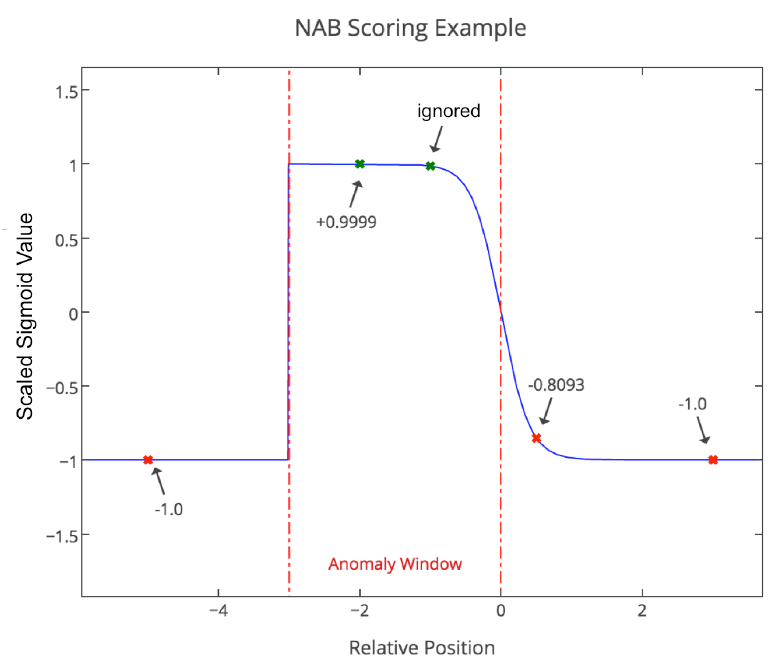
\includegraphics[width=0.7\linewidth]{ScoreExample.PNG}
\caption{Scoring example for a sample anomaly window, where the values represent the scaled sigmoid function. The first point is an FP preceding the anomaly window (red dashed lines) and contributes -1.0 to the score. Within the window, we see two detections, and only count the earliest TP for the score. There are two FPs after the window. The first is less detrimental because it is close to the window, and the second yields -1.0 because it's too far after the window to be associated with the true anomaly. TNs make no score contributions. The scaled sigmoid values are multiplied by the relevant application profile weight, the NAB score for this example would calculate as \( -1.0 A_{FP} + 0.9999 A_{TP} - 0.8093 A_{FP} - 1.0 A_{FP}\). With the standard application profile, this would result in a total score of 0.6909 \cite{7424283}}.
\label{fig:ScoringEx}
\end{figure}

\subsection{Data sets and function for displaying the results} \label{sec:display}

\pkg{Otsad} includes 51 of the 58 labeled one-dimensional time-series from different fields available in the NAB \cite{7424283} repository. Each of the datasets included in \pkg{otsad} is composed of three columns: the \emph{timestamp} column, the \emph{value} column and a third column called \emph{is.real.anomaly} containing the labeled truth anomalies.

Our package also includes a function called \textbf{PlotDetections} to display the detections results on a chart. This function by default returns an interactive graph, but it also has a choice to get a ggplot object and it could be edited.

\subsection{False positive reduction technique} \label{sec:fp}

Some algorithms already included techniques to reduce false positives. These can be only applied to the above algorithms. For this reason, we introduce and implement our own algorithm, \emph{ReduceAnomalies}, to reduce false positives, ensuring that it can be applied in all the algorithms. This algorithm is inspired by the real-life situation where a time-lapse exists between an alarm is triggered and until corrective action is taken. In other words, the minimum time lapse between the first and the second alarm. Our algorithm’s uses the number of processed data points between two detected anomalies to reduce the number of false positives. When the first anomaly $x_t$ is detected a new window of length $w$ is created, with $x_{t+1}$ as the starter point and $x_{t+w}$ as the endpoint. For each newly detected anomaly, its relative position compared to the window is evaluated. Detected anomalies inside the window are excluded. If a detected anomaly is outside the window, it is then considered as a real anomaly and new window is calculated in the same way as mentioned above.

\section{Use example}\label{sec:examplesec}

In this section we explain how to use the package. Section \ref{sec:installation} describes  how to install the package. In section \ref{sec:documentation} we show how to load the documentation. Then, section \ref{sec:examples} includes some examples to show how to use the package. Finally, section \ref{sec:summaryfunctions}

\subsection{Installation}\label{sec:installation}

The \pkg{otsad} package is available at GitHub repository, so it can be downloaded and installed directly from the R command line by typing:

\begin{knitrout}
\definecolor{shadecolor}{rgb}{0.969, 0.969, 0.969}\color{fgcolor}\begin{kframe}
\begin{alltt}
\hlkwd{install.packages}\hlstd{(}\hlstr{"devtools"}\hlstd{)}
\hlstd{devtools}\hlopt{::}\hlkwd{install_github}\hlstd{(}\hlstr{"alaineiturria/otsad"}\hlstd{)}
\end{alltt}
\end{kframe}
\end{knitrout}

To easily access all the package’s functions, it must be attached in the usual way:

\begin{knitrout}
\definecolor{shadecolor}{rgb}{0.969, 0.969, 0.969}\color{fgcolor}\begin{kframe}
\begin{alltt}
\hlkwd{library}\hlstd{(otsad)}
\end{alltt}
\end{kframe}
\end{knitrout}

\textbf{Special note: }

CAD-OSE executes a python script so it is necessary to have python2 or python3 installed. In addition, to get the same results in all operating systems it is necessary to have installed the hashlib and bencode-python3 python libraries.

\subsection{Documentation}\label{sec:documentation}

Considering that this vignette provides the user with an overview of the \pkg{otsad} package, it is also important to have access to the specific information of each of the available algorithms. This information can be checked in the documentation page corresponding to each algorithm. In all cases, the documentation has the same structure, consisting of the following sections (see Figure \ref{fig:documentation} for an example):

\begin{itemize}
\item A \emph{description} section, which gives a brief description of what the algorithm consists of (like those given in Section \ref{sec:package}).
\item A \emph{usage} section, where an overview of the function with the available parameters is given.
\item An \emph{arguments} section, where each of the input parameters is described.
\item A \emph{details} section, which provides the user with more details on the algorithm, conditions and recommendations on the values that can be taken by each of the input parameters.
\item A \emph{value} section, where the output parameters of the function are described.
\item A \emph{references} section that points to the original contribution where the detector(s) was proposed, where further details, motivations or contextualization can be found.
\item An \emph{examples} section, where one or more examples of the use of the functions are shown.
\end{itemize}

As usual in R, the documentation pages for each function can be loaded from the command line with the commands \code{?} or \code{help}:

\begin{knitrout}
\definecolor{shadecolor}{rgb}{0.969, 0.969, 0.969}\color{fgcolor}\begin{kframe}
\begin{alltt}
\hlopt{?}\hlstd{CpSdEwma}
\hlkwd{help}\hlstd{(CpSdEwma)}
\end{alltt}
\end{kframe}
\end{knitrout}

In addition, a user manual is available in the github repository of the  \pkg{otsad} package, which contains the complete documentation of the package and its functions.

\begin{figure}[htbp]
\centering
\includegraphics[width=0.5\linewidth]{documentationExample.png}
\caption{Extract from CpSdEwma detectors documentation page, showing the highlighted above aspects.}
\label{fig:documentation}
\end{figure}

\newpage

\subsection{Examples}\label{sec:examples}

Here is an example of how to solve a simple problem using SD-EWMA algorithm. The data has been generated as follows:

\begin{knitrout}
\definecolor{shadecolor}{rgb}{0.969, 0.969, 0.969}\color{fgcolor}\begin{kframe}
\begin{alltt}
\hlcom{## Generate data}
\hlkwd{set.seed}\hlstd{(}\hlnum{100}\hlstd{)}
\hlstd{n} \hlkwb{<-} \hlnum{500}
\hlstd{x} \hlkwb{<-} \hlkwd{sample}\hlstd{(}\hlnum{1}\hlopt{:}\hlnum{100}\hlstd{, n,} \hlkwc{replace} \hlstd{=} \hlnum{TRUE}\hlstd{)}
\hlstd{x[}\hlnum{70}\hlopt{:}\hlnum{90}\hlstd{]} \hlkwb{<-} \hlkwd{sample}\hlstd{(}\hlnum{110}\hlopt{:}\hlnum{115}\hlstd{,} \hlnum{21}\hlstd{,} \hlkwc{replace} \hlstd{=} \hlnum{TRUE}\hlstd{)} \hlcom{# distributional shift}
\hlstd{x[}\hlnum{25}\hlstd{]} \hlkwb{<-} \hlnum{200} \hlcom{# abrupt transient anomaly}
\hlstd{x[}\hlnum{320}\hlstd{]} \hlkwb{<-} \hlnum{170} \hlcom{# abrupt transient anomaly}
\hlstd{df} \hlkwb{<-} \hlkwd{data.frame}\hlstd{(}\hlkwc{timestamp} \hlstd{=} \hlnum{1}\hlopt{:}\hlstd{n,} \hlkwc{value} \hlstd{= x)}
\end{alltt}
\end{kframe}
\end{knitrout}

We can visualize the time-series as in Figure \ref{fig:ts} by typing:
\begin{knitrout}
\definecolor{shadecolor}{rgb}{0.969, 0.969, 0.969}\color{fgcolor}\begin{kframe}
\begin{alltt}
\hlkwd{plot}\hlstd{(}\hlkwc{x} \hlstd{= df}\hlopt{$}\hlstd{timestamp,} \hlkwc{y} \hlstd{= df}\hlopt{$}\hlstd{value,} \hlkwc{type} \hlstd{=} \hlstr{"l"}\hlstd{,}
     \hlkwc{main} \hlstd{=} \hlstr{"Time-Serie"}\hlstd{,} \hlkwc{col} \hlstd{=} \hlstr{"blue"}\hlstd{,} \hlkwc{xlab} \hlstd{=} \hlstr{"Time"}\hlstd{,} \hlkwc{ylab} \hlstd{=} \hlstr{"Value"}\hlstd{)}
\end{alltt}
\end{kframe}
\end{knitrout}

\begin{figure}[htbp]
\centering
\includegraphics[width=0.7\linewidth]{timeSerie.PNG}
\caption{Our time-series visualization}
\label{fig:ts}
\end{figure}


The SD-EWMA algorithm is designed for stationary time-series. Therefore, we must first check that the time-series is stationary. To do this, we can display the acf and pacf graphics (Figure \ref{fig:acf}) by:

\begin{knitrout}
\definecolor{shadecolor}{rgb}{0.969, 0.969, 0.969}\color{fgcolor}\begin{kframe}
\begin{alltt}
\hlstd{forecast}\hlopt{::}\hlkwd{Acf}\hlstd{(}\hlkwd{ts}\hlstd{(df}\hlopt{$}\hlstd{value),} \hlkwc{main} \hlstd{=} \hlstr{"ACF"}\hlstd{,} \hlkwc{lag} \hlstd{=} \hlnum{20}\hlstd{)}
\hlstd{forecast}\hlopt{::}\hlkwd{Pacf}\hlstd{(}\hlkwd{ts}\hlstd{(df}\hlopt{$}\hlstd{value),} \hlkwc{main} \hlstd{=} \hlstr{"PACF"}\hlstd{,} \hlkwc{lag} \hlstd{=} \hlnum{20}\hlstd{)}
\end{alltt}
\end{kframe}
\end{knitrout}

\begin{figure}[htbp]
\centering
\includegraphics[width=0.7\linewidth]{acf.PNG}
\caption{ACF and PACF graphs}
\label{fig:acf}
\end{figure}

We can observe that since almost all the lags are within the limits, the time-series is stationary. In addition, we can use two statistical tests, adf test and kpss test. The tests also indicate that the time-series is stationary.

\begin{knitrout}
\definecolor{shadecolor}{rgb}{0.969, 0.969, 0.969}\color{fgcolor}\begin{kframe}
\begin{alltt}
\hlkwd{library}\hlstd{(tseries)}
\hlkwd{adf.test}\hlstd{(df}\hlopt{$}\hlstd{value,} \hlkwc{alternative} \hlstd{=} \hlstr{'stationary'}\hlstd{,} \hlkwc{k} \hlstd{=} \hlnum{0}\hlstd{)}
\hlkwd{kpss.test}\hlstd{(df}\hlopt{$}\hlstd{value)}
\end{alltt}
\end{kframe}
\end{knitrout}

On the recommendation of the algorithm authors we set \code{threshold} to 0.01.One of the usual values for the $\sigma$ multiplier \code{l} is usually 3. Next, we apply the SD-EWMA anomaly detector, as the example is simple we use the classical processing algorithm. Note that the optimized algorithm could be used in the same way. Finally, we separate the training and test sets, using the first five values for training and the rest values for testing.

\begin{knitrout}
\definecolor{shadecolor}{rgb}{0.969, 0.969, 0.969}\color{fgcolor}\begin{kframe}
\begin{alltt}
\hlstd{result} \hlkwb{<-} \hlkwd{CpSdEwma}\hlstd{(}\hlkwc{data} \hlstd{= df}\hlopt{$}\hlstd{value,} \hlkwc{n.train} \hlstd{=} \hlnum{5}\hlstd{,} \hlkwc{threshold} \hlstd{=} \hlnum{0.01}\hlstd{,} \hlkwc{l} \hlstd{=} \hlnum{3}\hlstd{)}
\end{alltt}
\end{kframe}
\end{knitrout}

This results are of data.frame type and have three columns: \emph{is.anomaly} indicating whether or not the test observation is anomalous and the columns \emph{ucl} and \emph{lcl} with the upper and lower control limits, used to determine whether or not the observation is anomalous.

\begin{knitrout}
\definecolor{shadecolor}{rgb}{0.969, 0.969, 0.969}\color{fgcolor}\begin{kframe}
\begin{alltt}
\hlkwd{head}\hlstd{(result,} \hlkwc{n} \hlstd{=} \hlnum{15}\hlstd{)}
\end{alltt}
\begin{verbatim}
##    is.anomaly         lcl      ucl
## 1           0  74.0000000  74.0000
## 2           0  89.0000000  89.0000
## 3           0  78.0000000  78.0000
## 4           0  23.0000000  23.0000
## 5           0  86.0000000  86.0000
## 6           0   0.2998149 139.0313
## 7           0   0.6808881 138.7171
## 8           0  -8.3155413 134.5737
## 9           0  -8.8121491 133.4445
## 10          0  -7.7247629 133.8939
## 11          0  -4.6526720 137.8049
## 12          0 -12.4721436 133.7091
## 13          0 -19.2253248 129.7386
## 14          0 -18.8776837 129.3396
## 15          0 -19.8205462 127.8363
\end{verbatim}
\end{kframe}
\end{knitrout}

Finally, we can plot the results (Figure \ref{fig:result}) by writing the following code:

\begin{knitrout}
\definecolor{shadecolor}{rgb}{0.969, 0.969, 0.969}\color{fgcolor}\begin{kframe}
\begin{alltt}
\hlstd{res} \hlkwb{<-} \hlkwd{cbind}\hlstd{(df, result)}
\hlkwd{PlotDetections}\hlstd{(res,} \hlkwc{title} \hlstd{=} \hlstr{"KNN-CAD ANOMALY DETECTOR"}\hlstd{)}
\end{alltt}
\end{kframe}
\end{knitrout}

\begin{figure}[htbp]
\centering
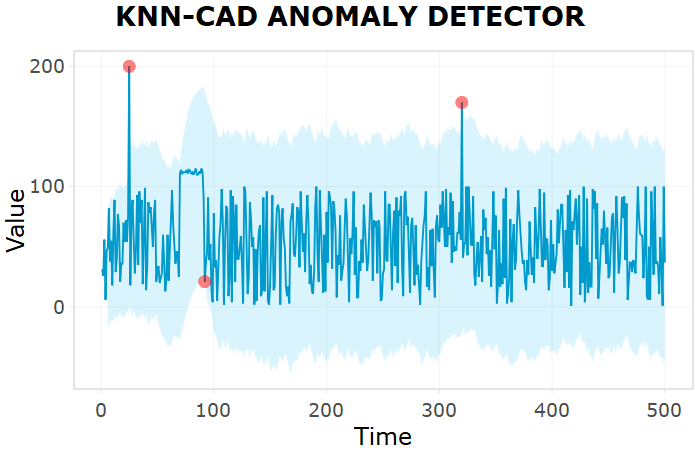
\includegraphics[width=0.5\linewidth]{sdEwmaresult.PNG}
\caption{Sd-Ewma Anomaly detector results}
\label{fig:result}
\end{figure}

In Figure \ref{fig:result} we can see that the detector has detected well both abrupt transient anomalies  and distributional shift anomaly.

This example has used classical processing, but by using the incremental function we can simulate online processing as follows:

\begin{knitrout}
\definecolor{shadecolor}{rgb}{0.969, 0.969, 0.969}\color{fgcolor}\begin{kframe}
\begin{alltt}
\hlcom{## Initialize parameters for the loop}
\hlstd{last.res} \hlkwb{<-} \hlkwa{NULL}
\hlstd{res} \hlkwb{<-} \hlkwa{NULL}
\hlstd{nread} \hlkwb{<-} \hlnum{250}
\hlstd{numIter} \hlkwb{<-} \hlstd{n}\hlopt\hlstd{nread}
\hlstd{iter} \hlkwb{<-} \hlkwd{seq}\hlstd{(}\hlnum{1}\hlstd{, nread} \hlopt{*} \hlstd{numIter, nread)}

\hlcom{## Calculate anomalies}
\hlkwa{for}\hlstd{(i} \hlkwa{in} \hlstd{iter) \{}
  \hlcom{# read new data}
  \hlstd{newRow} \hlkwb{<-} \hlstd{df[i}\hlopt{:}\hlstd{(i} \hlopt{+} \hlstd{nread} \hlopt{-} \hlnum{1}\hlstd{),]}
  \hlcom{# calculate if it's an anomaly}
  \hlstd{last.res} \hlkwb{<-} \hlkwd{IpSdEwma}\hlstd{(}
    \hlkwc{data} \hlstd{= newRow}\hlopt{$}\hlstd{value,}
    \hlkwc{n.train} \hlstd{=} \hlnum{5}\hlstd{,}
    \hlkwc{threshold} \hlstd{=} \hlnum{0.01}\hlstd{,}
    \hlkwc{l} \hlstd{=} \hlnum{3}\hlstd{,}
    \hlkwc{last.res} \hlstd{= last.res}\hlopt{$}\hlstd{last.res}
  \hlstd{)}
  \hlcom{# prepare the result}
  \hlkwa{if}\hlstd{(}\hlopt{!}\hlkwd{is.null}\hlstd{(last.res}\hlopt{$}\hlstd{result))\{}
    \hlstd{res} \hlkwb{<-} \hlkwd{rbind}\hlstd{(res,} \hlkwd{cbind}\hlstd{(newRow, last.res}\hlopt{$}\hlstd{result))}
  \hlstd{\}}
\hlstd{\}}
\end{alltt}
\end{kframe}
\end{knitrout}

In the same way we can plot the results (Figure ref{fig:result2}) by writing:

\begin{knitrout}
\definecolor{shadecolor}{rgb}{0.969, 0.969, 0.969}\color{fgcolor}\begin{kframe}
\begin{alltt}
\hlkwd{PlotDetections}\hlstd{(res,} \hlkwc{title} \hlstd{=} \hlstr{"SD-EWMA ANOMALY DETECTOR"}\hlstd{)}
\end{alltt}
\end{kframe}
\end{knitrout}

\begin{figure}[htbp]
\centering
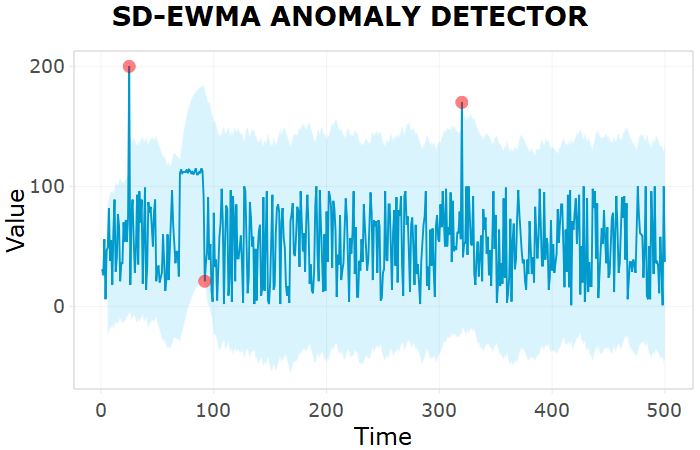
\includegraphics[width=0.5\linewidth]{onlineSdEwma.PNG}
\caption{Online Sd-Ewma Anomaly detector results}
\label{fig:result2}
\end{figure}

The use of the Contextual Anomaly detector is similar to the use of the previous algorithms. It is important to note that if the bencode python module is not installed, this method will rise an error. This can be prevented installing the bencode-pyhthon3 library with Python package manager \code{pip}.

\begin{knitrout}
\definecolor{shadecolor}{rgb}{0.969, 0.969, 0.969}\color{fgcolor}\begin{kframe}
\begin{alltt}
\hlstd{cad.results} \hlkwb{<-} \hlkwd{ContextualAnomalyDetector}\hlstd{(}
  \hlstd{df}\hlopt{$}\hlstd{value[}\hlnum{1}\hlopt{:}\hlnum{250}\hlstd{],}
  \hlkwc{base.threshold} \hlstd{=} \hlnum{0.75}\hlstd{,}
  \hlkwc{rest.period} \hlstd{=} \hlnum{5}\hlstd{,}
  \hlkwc{max.value} \hlstd{=} \hlnum{200}\hlstd{,}
  \hlkwc{min.value} \hlstd{=} \hlnum{0}
\hlstd{)}
\hlstd{cad.results.online} \hlkwb{<-} \hlkwd{ContextualAnomalyDetector}\hlstd{(}
  \hlstd{df}\hlopt{$}\hlstd{value[}\hlnum{251}\hlopt{:}\hlnum{500}\hlstd{],}
  \hlkwc{python.object} \hlstd{= cad.results}\hlopt{$}\hlstd{python.Object}
\hlstd{)}

\hlstd{res} \hlkwb{<-} \hlkwd{cbind}\hlstd{(df,} \hlkwd{rbind}\hlstd{(cad.results}\hlopt{$}\hlstd{result, cad.results.online}\hlopt{$}\hlstd{result))}
\hlkwd{PlotDetections}\hlstd{(res,} \hlkwc{title} \hlstd{=} \hlstr{"CONTEXTUAL ANOMALY DETECTOR"}\hlstd{)}
\end{alltt}
\end{kframe}
\end{knitrout}

\begin{figure}[htbp]
\centering
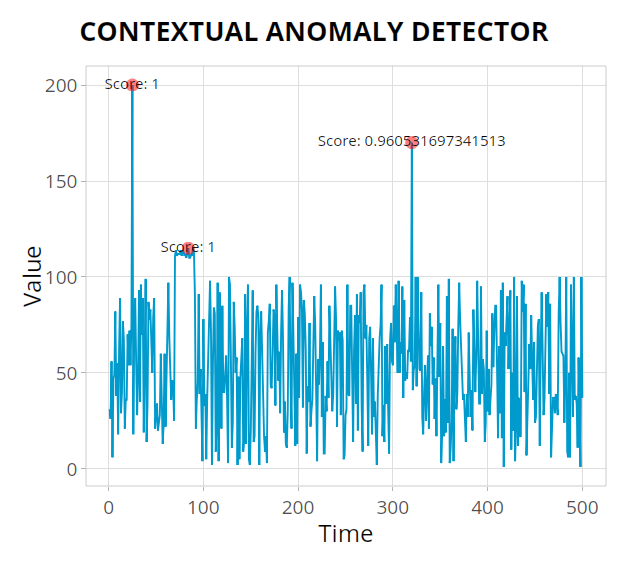
\includegraphics[width=0.5\linewidth]{cadose.PNG}
\caption{Contextual Anomaly Detector results}
\label{fig:cad}
\end{figure}

Finally we show a complete example using a data set included in the package. For this example, we used the \emph{Speed\_7578} dataset included in the package which has five anomalies. We used the KNN algorithm to try to find those anomalies.

\begin{knitrout}
\definecolor{shadecolor}{rgb}{0.969, 0.969, 0.969}\color{fgcolor}\begin{kframe}
\begin{alltt}
\hlcom{# Load the previously installed otsad package}
\hlkwd{library}\hlstd{(}\hlstr{"otsad"}\hlstd{)}

\hlcom{# Load the dataset speed_7578, included in otsad}
\hlstd{myData} \hlkwb{<-} \hlstd{speed_7578}

\hlcom{# Initialize parameters}
\hlstd{n} \hlkwb{<-} \hlkwd{nrow}\hlstd{(myData)}
\hlstd{n.train} \hlkwb{<-} \hlkwd{GetNumTrainingValues}\hlstd{(n)}

\hlcom{# Calculate anomalies using KNN-CAD}
\hlstd{result} \hlkwb{<-} \hlkwd{CpKnnCad}\hlstd{(}
  \hlkwc{data} \hlstd{= myData}\hlopt{$}\hlstd{value,}
  \hlkwc{n.train} \hlstd{= n.train,}
  \hlkwc{threshold} \hlstd{=} \hlnum{1}\hlstd{,}
  \hlkwc{l} \hlstd{=} \hlnum{19}\hlstd{,}
  \hlkwc{k} \hlstd{=} \hlnum{27}\hlstd{,}
  \hlkwc{ncm.type} \hlstd{=} \hlstr{"ICAD"}\hlstd{,}
  \hlkwc{reducefp} \hlstd{=} \hlnum{TRUE}
\hlstd{)}

\hlcom{# Add results to dataset}
\hlstd{myData} \hlkwb{<-} \hlkwd{cbind}\hlstd{(myData, result)}
\end{alltt}
\end{kframe}
\end{knitrout}

Once the algorithm is applied, we could show the results using the PlotDetections function. Since the resulting graph is interactive, in Figure \ref{fig:Example1Score} we show a capture of it.

\begin{knitrout}
\definecolor{shadecolor}{rgb}{0.969, 0.969, 0.969}\color{fgcolor}\begin{kframe}
\begin{alltt}
\hlcom{# Plot Results}
\hlkwd{PlotDetections}\hlstd{(myData,} \hlkwc{title} \hlstd{=} \hlstr{"KNN-CAD ANOMALY DETECTOR"}\hlstd{)}
\end{alltt}
\end{kframe}
\end{knitrout}

\begin{figure}[htbp]
\centering
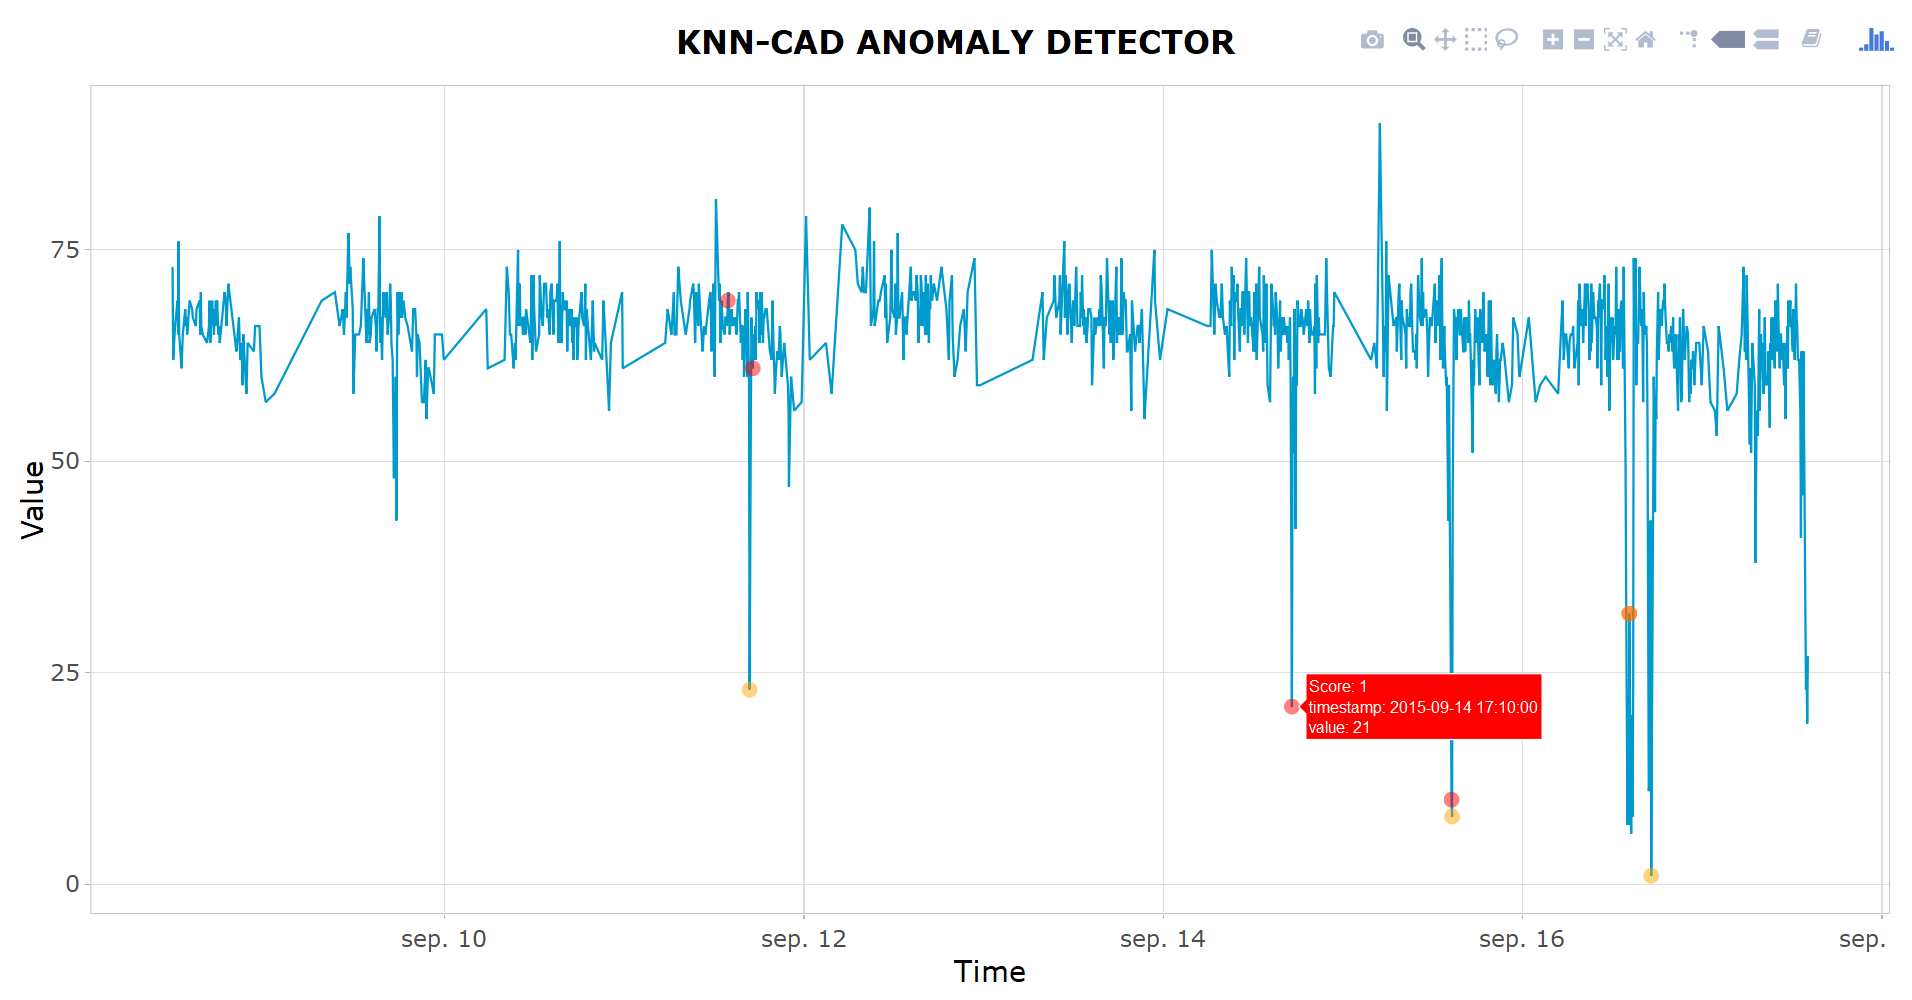
\includegraphics[width=1\linewidth]{Example1Score.PNG}
\caption{Anomalies detected in speed\_7578 dataset by KNN\_CAD detector.}
\label{fig:Example1Score}
\end{figure}


Next, we get the detector's score.

\begin{knitrout}
\definecolor{shadecolor}{rgb}{0.969, 0.969, 0.969}\color{fgcolor}\begin{kframe}
\begin{alltt}
\hlcom{# Get detector score}
\hlstd{score} \hlkwb{<-} \hlkwd{GetDetectorScore}\hlstd{(myData)}

\hlcom{# See this results}
\hlkwd{data.frame}\hlstd{(score[}\hlopt{-}\hlnum{1}\hlstd{])}
\end{alltt}
\end{kframe}
\end{knitrout}

This function has an option to show the results on a chart by adding the following parameters, see \ref{fig:Ej1ScoreDe}.

\begin{knitrout}
\definecolor{shadecolor}{rgb}{0.969, 0.969, 0.969}\color{fgcolor}\begin{kframe}
\begin{alltt}
\hlcom{# Get detector score}
\hlstd{score} \hlkwb{<-} \hlkwd{GetDetectorScore}\hlstd{(}
  \hlstd{myData,}
  \hlkwc{print} \hlstd{=} \hlnum{TRUE}\hlstd{,}
  \hlkwc{title} \hlstd{=} \hlstr{"speed_7578 results using KNN-CAD detector"}
\hlstd{)}
\end{alltt}
\end{kframe}
\end{knitrout}

\begin{figure}[htbp]
\centering
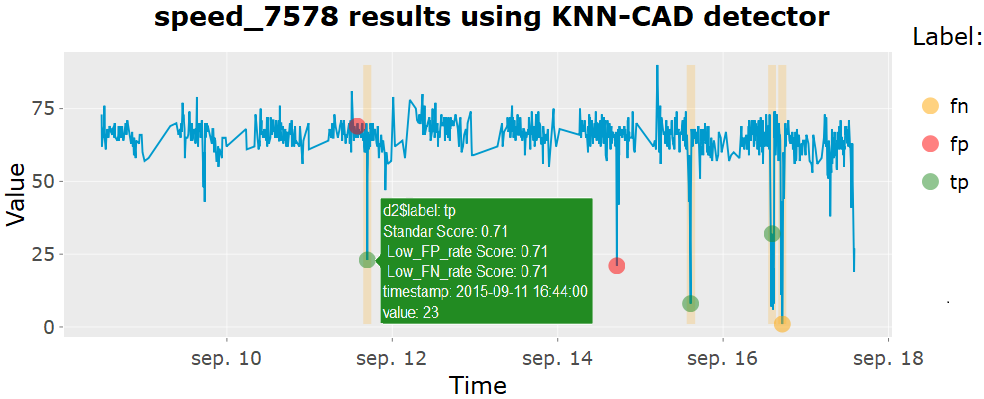
\includegraphics[width=1\linewidth]{Ej1ScoreDe.PNG}
\caption{KNN-CAD detector measurement results for speed\_7578 dataset.}
\label{fig:Ej1ScoreDe}
\end{figure}

Finally, we normalize the scores and show them.

\begin{knitrout}
\definecolor{shadecolor}{rgb}{0.969, 0.969, 0.969}\color{fgcolor}\begin{kframe}
\begin{alltt}
\hlcom{# Normalize results}
\hlstd{null.perfect} \hlkwb{<-} \hlkwd{GetNullAndPerfectScores}\hlstd{(myData)}

\hlstd{standar.score} \hlkwb{<-} \hlkwd{NormalizeScore}\hlstd{(}
  \hlstd{score}\hlopt{$}\hlstd{standard,}
  \hlkwc{perfect.score} \hlstd{= null.perfect[}\hlnum{1}\hlstd{,} \hlstr{"perfect.score"}\hlstd{],}
  \hlkwc{null.score} \hlstd{= null.perfect[}\hlnum{1}\hlstd{,} \hlstr{"null.score"}\hlstd{]}
\hlstd{)}

\hlstd{low_FP_rate.score} \hlkwb{<-} \hlkwd{NormalizeScore}\hlstd{(}
  \hlstd{score}\hlopt{$}\hlstd{low_FP_rate,}
  \hlkwc{perfect.score} \hlstd{= null.perfect[}\hlnum{2}\hlstd{,} \hlstr{"perfect.score"}\hlstd{],}
  \hlkwc{null.score} \hlstd{= null.perfect[}\hlnum{2}\hlstd{,} \hlstr{"null.score"}\hlstd{]}
\hlstd{)}

\hlstd{low_FN_rate.score} \hlkwb{<-} \hlkwd{NormalizeScore}\hlstd{(}
  \hlstd{score}\hlopt{$}\hlstd{low_FN_rate,}
  \hlkwc{perfect.score} \hlstd{= null.perfect[}\hlnum{3}\hlstd{,} \hlstr{"perfect.score"}\hlstd{],}
  \hlkwc{null.score} \hlstd{= null.perfect[}\hlnum{3}\hlstd{,} \hlstr{"null.score"}\hlstd{]}
\hlstd{)}

\hlcom{# Show normalized scores}
\hlkwd{cbind}\hlstd{(standar.score, low_FP_rate.score, low_FN_rate.score)}
\end{alltt}
\end{kframe}
\end{knitrout}

\subsection{Most useful functions}
\label{sec:summaryfunctions}

\begin{table}[htbp]
  \centering
  \resizebox{\textwidth}{!}{%
  \begin{tabular}{llll}
    \hline
    \textbf{Functionality} & \textbf{Description} & \textbf{Offline} & \textbf{Online} \\ \hline
    \multirow{6}{*}{Detectors} & PEWMA & CpPewma & IpPewma \\
     & SD-EWMA & CpSdEwma & IpSdEwma \\
     & TSSD-EWMA & CpTsSdEwma & IpTsSdEwma \\
     & KNN-ICAD & CpKnnCad(ncm.type = "ICAD") & IpKnnCad(ncm.type = "ICAD") \\
     & KNN-LDCD & CpKnnCad(ncm.type = "LDCD") & IpKnnCad(ncm.type = "LDCD") \\
     & CAD-OSE & ContextualAnomalyDetector & ContextualAnomalyDetector \\ \hline
    \multirow{2}{*}{NAB score} & Get score & GetDetectorScore & \multicolumn{1}{c}{-} \\
     & Normalize score: & \begin{tabular}[c]{@{}l@{}}NormalizeScore\\
     GetNullAndPerfectScores\end{tabular} & \multicolumn{1}{c}{-} \\ \hline
    \begin{tabular}[c]{@{}l@{}}False Positve \\
    Reduction\end{tabular} & False positive reduction & ReduceAnomalies & ReduceAnomalies \\ \hline
    Visualization & \begin{tabular}[c]{@{}l@{}}Static or \\
    interactive visualizations\end{tabular} & PlotDetections & \multicolumn{1}{c}{-} \\ \hline
  \end{tabular}%
  }
\end{table}

\section{Summary}\label{sec:summary}

In this paper, we present the \pkg{otsad} package for R. This package fully meets the demand for anomaly detection algorithms over univariate time series in online environments. With this package we tackle with the ability to work with stationary and non-stationary data. We also provide algorithms of the two detection techniques (evolving and window based) that are gaining strength on research.

As a future job, we propose to maintain and add functionalities to our \pkg{otsad} package, i.e. provide more sophisticated false positive reduction techniques and incorporate them into algorithms.

\bibliography{otsad}
\bibliographystyle{plain}

\end{document}
